\begin{Example}[soccer2]{UK Soccer scores}
In \exref{ex:soccer}, we examined the distribution of goals scored
by the home team and the away team in 380 games in the 1995/96 season
by the 20 teams in the UK Football Association, Premier League.
The analysis there focused on the distribution of the total goals
scored, under the assumption that the number of goals scored by
the home team and the away team were independent.

Here we test that assumption and illustrate the simple use of the
\macro{MOSAIC} to construct the mosaic display.
It turns out that independence does in fact hold, and the
resulting graph also illustrates a typical pattern
shown under independence.

The \Dstp{} \texttt{soccer} below reads the data from \tabref{tab:soccer1}
in the same way as in \exref{ex:soccer}, producing a \Dset\
with a frequency variable \pname{freq} and factor variables
\pname{home} and \pname{away}.
The \macro{MOSAIC} reads this \Dset\ into \IML{}, and runs
the \texttt{mosaics} module,
The \mparm{plots=2}{MOSAIC} causes the program to display only the
mosaic plot for the two-way table.

\begin{table}[!hb]
\caption{Total goals scored in 380 games in the Premier
Football League, 1995/95 season}
\label{tab:soccer2}
\vspace{.1in}
\begin{center}
\begin{tabular}{l|rrrr rrrr}
\hline
Total goals      &  0  &  1  &  2  &  3  &  4  &  5  &  6  &  7  \\
\hline
Number of games  & 27  & 88  & 91  & 73  & 49  & 31  & 18  &  3  \\
  \hline
\end{tabular}
\end{center}
\end{table}


The printed output (not shown) gives the Pearson \chisq{} as
18.7 with 16 df, indicating that home and away goals are independent.
\figref{fig:soccer2} shows the mosaic display.
The tiles in each row are approximately
the same height, and all the tiles except one are unshaded.
\begin{figure}[htb]
  \centering
  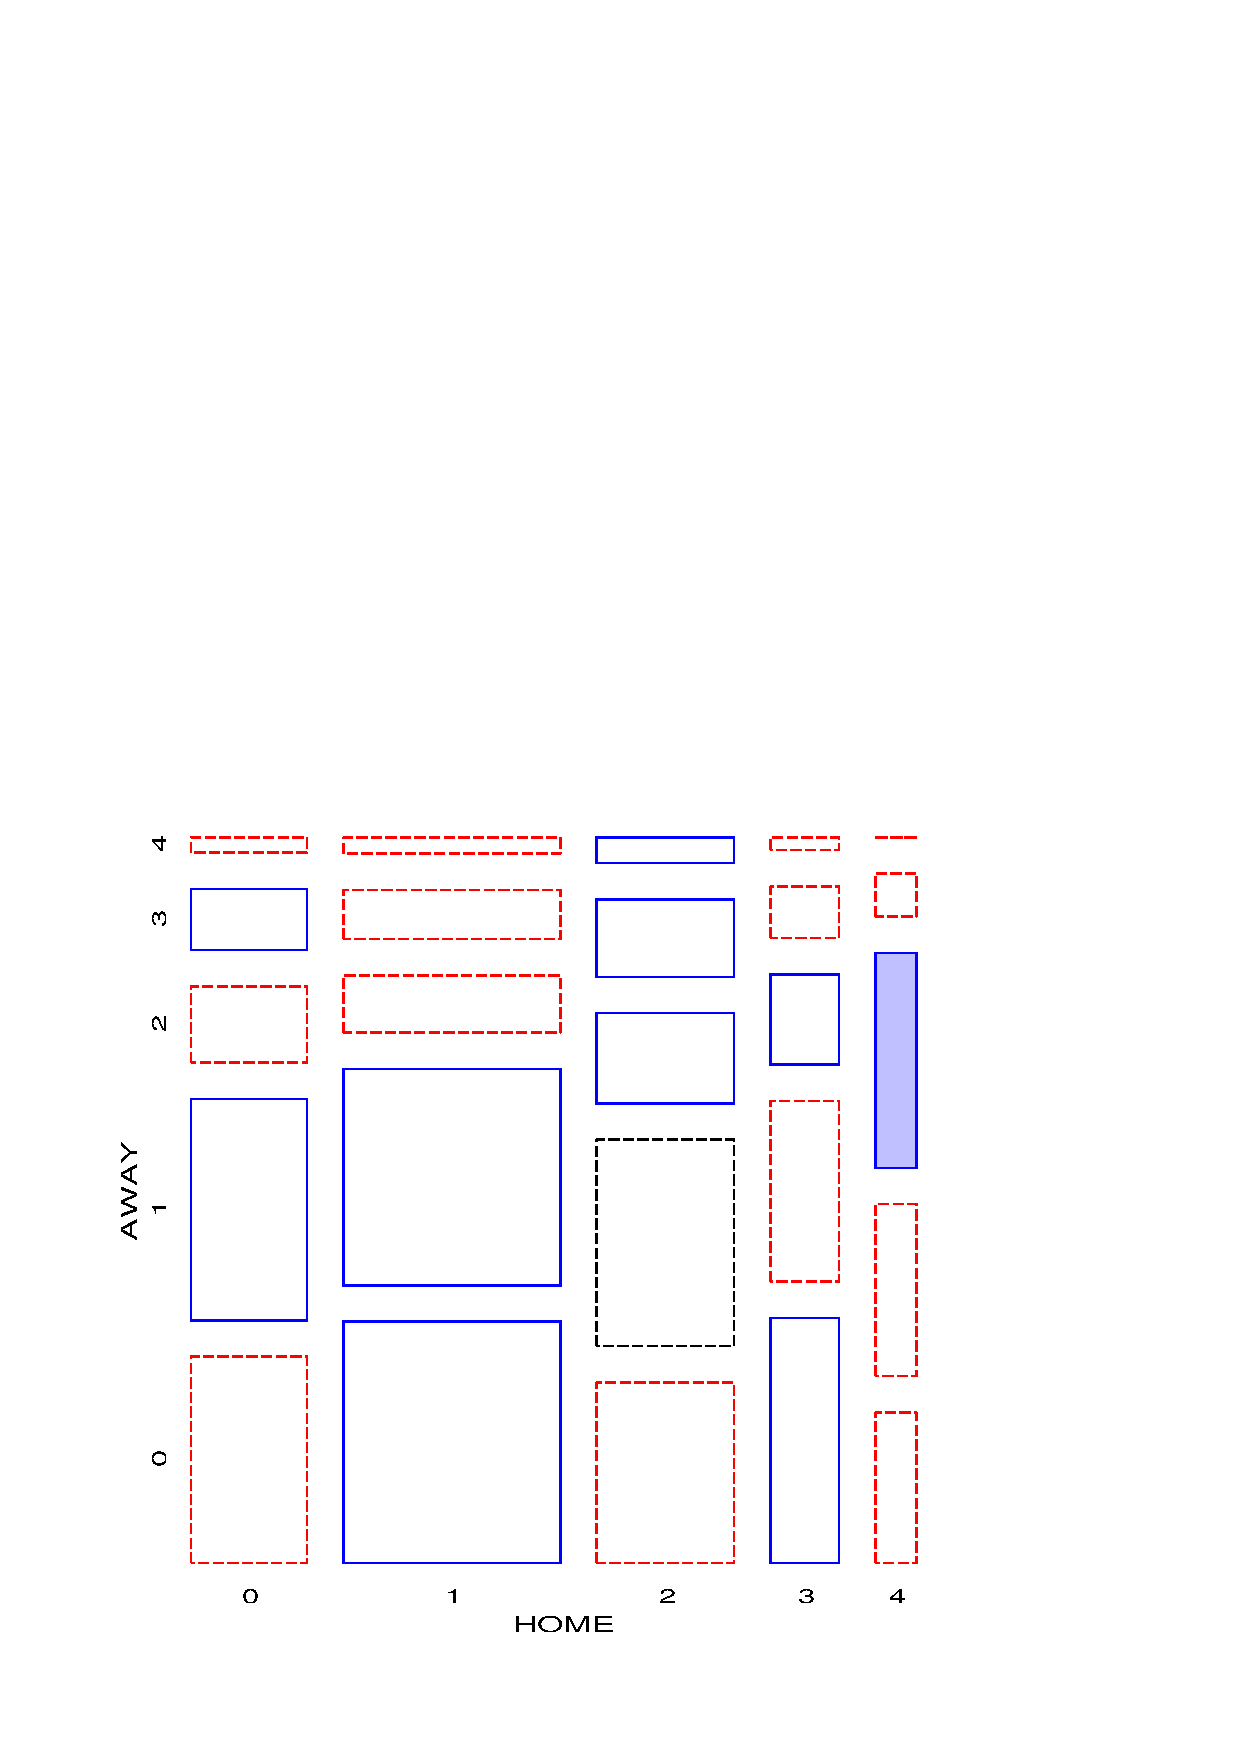
\includegraphics[scale=.6]{ch4/fig/soccer2}
  \caption[Mosaic display for UK Soccer scores]{Mosaic display for UK Soccer scores}  \label{fig:soccer2}
\end{figure}

The one exception is for the situation where the home team scores
four or more goals, and the away team scores two goals, which occurs
more often than one would predict under independence.
This residual ($d_{42} = 3.08$) accounts for nearly half of the overall
\chisq{}.
It may or may not be unusual to find one moderately large residual
in a $5 \times 5$ table.
A half-normal plot of the residuals
(described in \secref{sec:loglin-halfnorm}),
plots the absolute values of residuals
against expected values of normal
order statistics, with a simulated 95\% envelope for residuals from a
good-fitting model.
This plot, shown in \figref{fig:soccer4}, suggests that the residual in
the $(4, 2)$ cell is not unduly large.


\begin{figure}[htb]
  \centering
  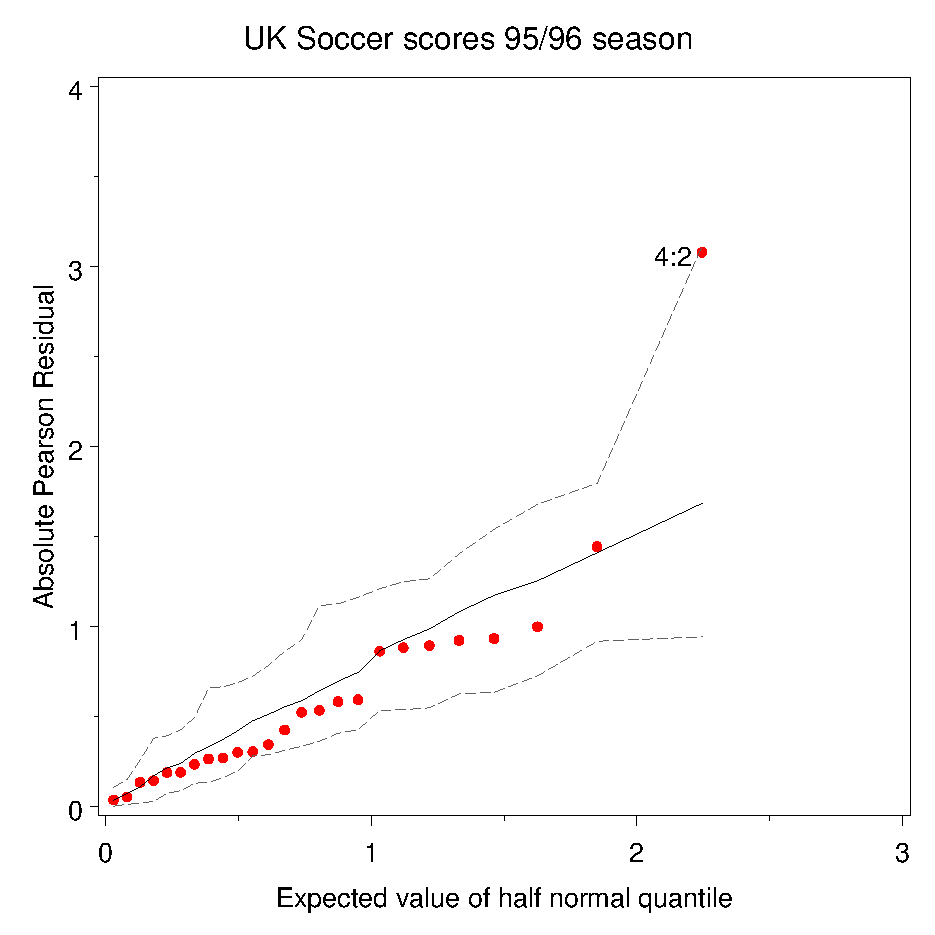
\includegraphics[scale=.6]{ch4/fig/soccer4}
  \caption[Half-normal plot for UK Soccer scores]{Half-normal plot for UK Soccer scores}\label{fig:soccer4}
\end{figure}
\end{Example}
